\documentclass[11pt]{article}

\usepackage[margin=1in]{geometry}
\usepackage{graphicx}
\usepackage{booktabs}
\usepackage{amsmath}
\usepackage{algorithm}
\usepackage{algpseudocode}
\usepackage[numbers,sort&compress]{natbib}
\usepackage[hidelinks]{hyperref}

\title{SWIFT (Smith-Waterman Algorithm with Intelligent Filtering and Tiling): A Parallel, K-mer Filtered Smith-Waterman Extension for Fast and Accurate Local Sequence Alignment}
\author{Prince Samuel Kyeremanteng \and Alexandra Naa Atwei Quao \and Christabel Agyemang}
\date{}

\begin{document}
\maketitle

\begin{abstract}
\textbf{Background:} Local sequence alignment remains a common bottleneck in genomics, transcriptomics, and metagenomics workflows. The Smith-Waterman dynamic programming recurrence is still attractive because it gives an optimal local alignment under the selected scoring scheme, but the full dynamic programming matrix is expensive to evaluate for large query-target pairs. Recent work has attacked this problem through SIMD execution, GPUs, FPGAs, processing-in-memory systems, sparse seeding, minimizers, and graph-aware chaining. These efforts make clear that speed is not one problem but several: the search space must be reduced, memory traffic must be controlled, and parallel work must be made coarse enough to pay for scheduling overhead.

\textbf{Results:} We present SWIFT, a lightweight CPU-parallel local alignment framework that combines rolling k-mer filtering, fixed-size target tiling, parallel Smith-Waterman alignment on candidate tiles, and a merge-and-refine pass. The method does not attempt to replace full dynamic programming in every case. Instead, it uses k-mer evidence to decide where full local alignment is worth spending. On the included representative DNA test case, the Python implementation reduced wall-clock time from 7.48 seconds for a single full Smith-Waterman pass to 3.88 seconds for the tiled parallel workflow, a 48.1\% reduction. The best raw tile score was smaller than the full alignment score, as expected, but the merge-and-refine stage recovered coherent local spans and exported results in JSON and SAM-like formats.

\textbf{Conclusions:} SWIFT appears most useful as an interpretable seed-filter-extend baseline for medium-scale experiments, teaching, and early prototyping where specialized hardware is unavailable. Its main weakness is also clear: sensitivity depends on k-mer size, tile size, and hit threshold, and repetitive sequences may over-select tiles. Still, the design suggests a practical middle ground between exact full-matrix alignment and highly engineered aligners.
\end{abstract}

\noindent\textbf{Keywords:} local sequence alignment; Smith-Waterman; k-mer filtering; tiling; parallel computing; seed-filter-extend; bioinformatics software

\section{Introduction}
Sequence alignment is one of those computational biology problems that never quite disappears. It sits under read mapping, homology search, assembly polishing, viral surveillance, pangenome analysis, and a long list of smaller laboratory tasks that need to compare two biological strings without pretending they are identical. The classical Smith-Waterman formulation is still a useful reference point because it computes the optimal local alignment under a chosen scoring model. The difficulty is familiar: filling an $m \times n$ matrix for a query of length $m$ and target of length $n$ scales poorly once either sequence becomes large.

Recent aligners have moved in several directions. Wavefront methods exploit the relationship between edit score and explored dynamic programming states \citep{marcosola2021wfa,aguadopuig2023wfagpu}. SIMD and block-based methods reshape the dynamic programming matrix so CPUs can do more work per instruction \citep{liu2023blockaligner}. GPU and FPGA designs push much harder on parallelism, sometimes reaching impressive cell-update rates, but often at the cost of a more demanding software or hardware stack \citep{schmidt2024cudasw4,aguadopuig2022wfa_gpu_access,alvarez2023wfafpga,perezwohlfeil2023gpu_irregular}. Processing-in-memory work has also made the memory-bandwidth limit hard to ignore \citep{diab2023aim,diab2022wfa_pim}. At the other end of the spectrum, seed selection, minimizers, and k-mer sketches try to avoid unnecessary alignment in the first place \citep{shaw2022local_kmer_selection,yu2024minimizers_filters,hoang2024masked_minimizer,marcais2024small_window,ndiaye2024minimizers_review}.

SWIFT (Smith-Waterman with Intelligent Filtering and Tiling) follows that second instinct. It assumes that many target regions are unlikely to produce useful local alignments, and it makes that assumption explicit: index the query's k-mers, count matching k-mers in target tiles, align only the tiles whose counts pass a threshold, then merge and refine candidate spans. This is not a claim that k-mer filtering is new. Rather, the contribution is a compact and inspectable pipeline that places k-mer filtering, tiling, multiprocessing, visualization, and JSON/SAM export into one reproducible Python implementation.

\section{Related Work}
\subsection{Parallel and hardware-accelerated dynamic programming}
Parallel Smith-Waterman implementations have been studied for years, but the last few years have been especially active because long-read sequencing, protein database growth, and pangenome analysis have changed the scale of routine alignment. \citet{xia2022parallel_sw_review} summarize the main parallelization strategies and their trade-offs. GPU-oriented approaches continue to be attractive because many independent alignment tasks can be batched, and because dynamic programming wavefronts expose regular computation when arranged carefully. CUDASW++4.0 is a good recent example: it combines matrix tiling, database partitioning, warp-level communication, and recent NVIDIA DPX features for protein database search \citep{schmidt2024cudasw4}. Other GPU studies show that performance depends not only on arithmetic throughput but also on irregular memory access, transfer overlap, and backtrace representation \citep{aguadopuig2022wfa_gpu_access,aguadopuig2023wfagpu,perezwohlfeil2023gpu_irregular,wang2024gpu_sw}.

Hardware specialization is not limited to GPUs. FPGA and sliding-window accelerator designs suggest that local alignment can benefit from systolic and streaming execution, especially where the input structure is predictable \citep{alvarez2023wfafpga,baik2023sliding_window_sw}. Processing-in-memory approaches attack a different bottleneck: the cost of moving dynamic programming state through the memory hierarchy \citep{diab2023aim,diab2022wfa_pim}. SWIFT is intentionally more modest. It uses ordinary CPU multiprocessing, but borrows the broader lesson that alignment work should be partitioned into independent units whenever possible.

\subsection{Seeds, minimizers, and filtered alignment}
The first question in many modern alignment workflows is not ``how do we align?'' but ``where should we even try?'' K-mer and minimizer schemes provide compact evidence of similarity and can reduce the number of expensive extensions. The theory of local k-mer selection helps explain why some seed-selection strategies preserve useful coverage better than others \citep{shaw2022local_kmer_selection}. Newer work on masked minimizers, decycling-set sketches, and minimizer reviews adds more nuance: low density and high conservation often pull against each other, and the best sketch depends on the error model and downstream task \citep{hoang2024masked_minimizer,marcais2024small_window,ndiaye2024minimizers_review,yu2024minimizers_filters}.

The same idea appears in applied aligners. X-Mapper uses gapped x-mers to balance seed length and mutation tolerance \citep{gaston2025xmapper}. Long-read mapping methods have also used variable k-mer ideas to handle noisy reads \citep{yang2021mapalign}. SWIFT currently uses exact contiguous k-mers, which is simple and fast, but less tolerant of substitutions and indels than spaced, syncmer, or gapped-seed designs. That limitation is acceptable for a first implementation, though it should be addressed in future versions.

\subsection{Graph and pangenome alignment context}
Although SWIFT is a pairwise linear-sequence method, recent pangenome work is relevant because it highlights where filtering and chaining have become essential. Sparse minimizer indexes, co-linear chaining, haplotype-aware graph alignment, and partial order alignment all try to avoid exhaustive comparison while preserving enough structure for accurate extension \citep{gao2024sigaligner,rajput2024colinear_chaining,chandra2024haplotype_graph_alignment,vandijk2025poasta}. These graph methods are more ambitious than SWIFT, but they reinforce the same basic point: exact dynamic programming is often best reserved for regions that have already earned attention.

\section{Methods}
\subsection{Algorithm overview}
SWIFT accepts a query sequence $Q$, target sequence $T$, k-mer length $k$, tile size $s$, and hit threshold $\tau$. The target is partitioned into fixed-length tiles. A tile becomes a candidate if at least $\tau$ of its k-mers appear in the query k-mer index. Candidate tiles are aligned independently against the full query using Smith-Waterman. The resulting tile-level alignments are converted into approximate query and target coordinates, sorted, merged where they overlap or touch, and refined by another Smith-Waterman pass on the merged spans.

\begin{figure}[ht]
  \centering
  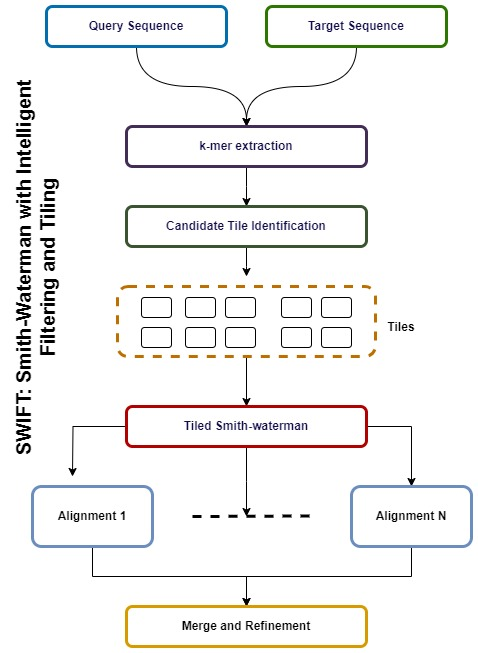
\includegraphics[width=0.68\linewidth]{images/swift-architecture.jpg}
  \caption{SWIFT workflow. Query and target sequences are reduced to k-mer evidence, target tiles with enough hits are selected, candidate tiles are aligned in parallel, and the resulting local alignments are merged and refined.}
  \label{fig:architecture}
\end{figure}

\begin{algorithm}[ht]
\caption{SWIFT local alignment workflow}
\begin{algorithmic}[1]
\Require Query $Q$, target $T$, k-mer length $k$, tile size $s$, hit threshold $\tau$
\Ensure Refined local alignments
\State $I \gets$ map from each k-mer in $Q$ to its query positions
\State $C \gets \emptyset$
\For{each k-mer position $i$ in $T$}
  \If{$T[i:i+k] \in I$}
    \State Increment the hit count of tile $\lfloor i/s \rfloor$
  \EndIf
\EndFor
\For{each tile with hit count $\geq \tau$}
  \State Add tile coordinates to $C$
\EndFor
\State Align each candidate tile in $C$ against $Q$ in parallel using Smith-Waterman
\State Convert tile alignments to approximate global coordinates
\State Merge overlapping or adjacent candidate spans
\State Refine each merged span with Smith-Waterman
\State Export alignment metadata, aligned strings, and optional visual summaries
\end{algorithmic}
\end{algorithm}

\subsection{Implementation}
The reference implementation is written in Python. Query k-mers are stored in a dictionary from k-mer string to positions. Candidate tile detection scans the target once and uses a set of query k-mers for membership checks. Tile alignment uses a NumPy-backed Smith-Waterman score matrix. Multiprocessing distributes independent candidate tiles across CPU workers. A separate pure-Python Smith-Waterman routine is used during merge/refine to recover local span boundaries.

The default parameters in the current implementation are $k=3$, $s=64$, and $\tau=2$. These defaults are deliberately small because the bundled example data are synthetic and relatively short. In real DNA or protein workloads, $k$ should usually be increased to reduce random hits; the right value depends on alphabet size, sequence length, expected divergence, and whether the user wants sensitivity or speed.

\subsection{Complexity}
Full Smith-Waterman requires $O(mn)$ time and $O(mn)$ memory for query length $m$ and target length $n$ if the entire score matrix is retained. SWIFT adds an $O(n)$ target scan after indexing the query. If candidate tiles cover $r$ target characters, the dominant alignment cost becomes approximately $O(mr)$, plus refinement over merged spans. In the worst case, especially on repetitive targets or very permissive thresholds, $r$ may approach $n$ and SWIFT reduces to full-matrix work with extra overhead. In the expected case, when k-mer filtering removes most of the target, $r \ll n$ and the method gains time from avoiding unpromising matrix cells.

\section{Experimental Setup}
The current evaluation uses the repository's bundled synthetic DNA query-target pair. Experiments were run with default parameters ($k=3$, tile size $64$, hit threshold $2$). The baseline was a single Smith-Waterman alignment of the full query against the full target using the same scoring choices: match $+2$, mismatch $-1$, and gap $-2$. The SWIFT run used all available CPU cores through Python multiprocessing.

This is a small evaluation, so the results should be read as a proof of behavior rather than a broad benchmark. A stronger evaluation would use controlled edit rates, real read sets, protein sequences, and comparisons against production aligners. Still, the bundled test is useful because it exercises the complete path: filtering, parallel tile alignment, merge/refine, visualization, JSON export, and SAM-like export.

\section{Results}
\begin{table}[ht]
\centering
\caption{Representative runtime from the bundled repository example.}
\label{tab:runtime}
\begin{tabular}{lrrr}
\toprule
Method & Runtime (s) & Best score & Units aligned \\
\midrule
Full Smith-Waterman & 7.48 & 1226 & 1 full target \\
SWIFT, parallel tiled & 3.88 & 128 & 75 candidate tiles \\
\bottomrule
\end{tabular}
\end{table}

The representative run reduced wall-clock time by 48.1\% relative to the full Smith-Waterman baseline (Table~\ref{tab:runtime}). That reduction is consistent with SWIFT's design: most target positions are never passed to dynamic programming. The best tile score is lower than the full Smith-Waterman score because each candidate tile sees only a local target window. This is not a failure by itself. The tile score is used as a ranking and filtering signal, while the merge/refine stage attempts to recover longer coherent regions.

The implementation also produced JSON and SAM-like outputs. JSON is useful for inspection because it stores alignment coordinates, scores, and aligned strings. SAM-style output makes the results easier to place near downstream genomics tools, although the current exporter is intentionally simple and should not be treated as a full SAM/BAM replacement.

\section{Discussion}
SWIFT's main advantage is its transparency. The algorithm can be explained in a few steps, each parameter has an obvious role, and intermediate results are easy to inspect. That is valuable for a research prototype. Many high-performance aligners are faster and more mature, but they also hide substantial engineering behind specialized kernels, vectorized libraries, or graph indexes. SWIFT instead asks a narrow question: how much work can be skipped before running local dynamic programming?

There are trade-offs. Small k-mers increase sensitivity but also increase random hits, especially in low-complexity or repetitive DNA. Larger k-mers reduce false positives but may miss alignments with substitutions or indels. Fixed non-overlapping tiles are simple, yet they can split a good alignment across boundaries. The merge/refine step repairs some of that damage, but boundary effects remain possible. Repetitive regions are another concern because many tiles can pass the threshold, reducing the expected speedup and possibly producing redundant candidate alignments.

Compared with recent GPU, SIMD, and wavefront methods, SWIFT is not trying to win peak throughput \citep{schmidt2024cudasw4,liu2023blockaligner,aguadopuig2023wfagpu}. Its likely niche is different: CPU-only environments, small laboratories, classrooms, or pipeline prototyping where interpretability matters and installing hardware-specific tools is inconvenient. A fair way to view SWIFT is as a seed-filter-extend scaffold that still uses Smith-Waterman at the extension stage.

\section{Limitations}
The present study has four important limitations. First, the benchmark is too small to support broad claims about runtime or accuracy. Second, exact contiguous k-mers are brittle under indel-rich errors. Third, the multiprocessing overhead may dominate on short sequences or when few tiles survive filtering. Fourth, the coordinate reconstruction from aligned tile strings is approximate enough that edge cases should be tested more heavily before clinical or production use.

\section{Future Work}
Several extensions are natural. Overlapping tiles would reduce boundary artifacts, though at some extra cost. Spaced seeds, syncmers, or gapped x-mers may improve sensitivity under realistic sequencing errors \citep{gaston2025xmapper,hoang2024masked_minimizer,shaw2022local_kmer_selection}. Adaptive tile sizes could use local hit density instead of a fixed window. A compiled alignment kernel, perhaps through Numba, Cython, Rust, or a SIMD library, would make the comparison with modern CPU aligners more meaningful. Finally, a larger benchmark should report not only runtime but also sensitivity, precision, identity, memory use, and behavior on repetitive targets.

\section{Conclusion}
SWIFT combines k-mer filtering, target tiling, parallel local alignment, and merge/refine reconstruction into a compact Smith-Waterman extension. The included example shows a clear runtime reduction while preserving an exact dynamic programming step for selected regions. The method is not a substitute for mature production aligners, and it does not remove the need for careful parameter tuning. It does, however, provide a useful and readable baseline for studying how much local alignment work can be avoided by simple sequence evidence before the dynamic programming matrix is built.

\section*{Availability}
The SWIFT implementation, example data, visualizations, LaTeX manuscript, BibTeX database, and notebook conversion are contained in the project repository.

\nocite{*}
\bibliographystyle{plainnat}
\bibliography{citations}

\end{document}
